% GNUPLOT: LaTeX picture with Postscript
\begingroup
  \makeatletter
  \providecommand\color[2][]{%
    \GenericError{(gnuplot) \space\space\space\@spaces}{%
      Package color not loaded in conjunction with
      terminal option `colourtext'%
    }{See the gnuplot documentation for explanation.%
    }{Either use 'blacktext' in gnuplot or load the package
      color.sty in LaTeX.}%
    \renewcommand\color[2][]{}%
  }%
  \providecommand\includegraphics[2][]{%
    \GenericError{(gnuplot) \space\space\space\@spaces}{%
      Package graphicx or graphics not loaded%
    }{See the gnuplot documentation for explanation.%
    }{The gnuplot epslatex terminal needs graphicx.sty or graphics.sty.}%
    \renewcommand\includegraphics[2][]{}%
  }%
  \providecommand\rotatebox[2]{#2}%
  \@ifundefined{ifGPcolor}{%
    \newif\ifGPcolor
    \GPcolortrue
  }{}%
  \@ifundefined{ifGPblacktext}{%
    \newif\ifGPblacktext
    \GPblacktextfalse
  }{}%
  % define a \g@addto@macro without @ in the name:
  \let\gplgaddtomacro\g@addto@macro
  % define empty templates for all commands taking text:
  \gdef\gplbacktext{}%
  \gdef\gplfronttext{}%
  \makeatother
  \ifGPblacktext
    % no textcolor at all
    \def\colorrgb#1{}%
    \def\colorgray#1{}%
  \else
    % gray or color?
    \ifGPcolor
      \def\colorrgb#1{\color[rgb]{#1}}%
      \def\colorgray#1{\color[gray]{#1}}%
      \expandafter\def\csname LTw\endcsname{\color{white}}%
      \expandafter\def\csname LTb\endcsname{\color{black}}%
      \expandafter\def\csname LTa\endcsname{\color{black}}%
      \expandafter\def\csname LT0\endcsname{\color[rgb]{1,0,0}}%
      \expandafter\def\csname LT1\endcsname{\color[rgb]{0,1,0}}%
      \expandafter\def\csname LT2\endcsname{\color[rgb]{0,0,1}}%
      \expandafter\def\csname LT3\endcsname{\color[rgb]{1,0,1}}%
      \expandafter\def\csname LT4\endcsname{\color[rgb]{0,1,1}}%
      \expandafter\def\csname LT5\endcsname{\color[rgb]{1,1,0}}%
      \expandafter\def\csname LT6\endcsname{\color[rgb]{0,0,0}}%
      \expandafter\def\csname LT7\endcsname{\color[rgb]{1,0.3,0}}%
      \expandafter\def\csname LT8\endcsname{\color[rgb]{0.5,0.5,0.5}}%
    \else
      % gray
      \def\colorrgb#1{\color{black}}%
      \def\colorgray#1{\color[gray]{#1}}%
      \expandafter\def\csname LTw\endcsname{\color{white}}%
      \expandafter\def\csname LTb\endcsname{\color{black}}%
      \expandafter\def\csname LTa\endcsname{\color{black}}%
      \expandafter\def\csname LT0\endcsname{\color{black}}%
      \expandafter\def\csname LT1\endcsname{\color{black}}%
      \expandafter\def\csname LT2\endcsname{\color{black}}%
      \expandafter\def\csname LT3\endcsname{\color{black}}%
      \expandafter\def\csname LT4\endcsname{\color{black}}%
      \expandafter\def\csname LT5\endcsname{\color{black}}%
      \expandafter\def\csname LT6\endcsname{\color{black}}%
      \expandafter\def\csname LT7\endcsname{\color{black}}%
      \expandafter\def\csname LT8\endcsname{\color{black}}%
    \fi
  \fi
    \setlength{\unitlength}{0.0500bp}%
    \ifx\gptboxheight\undefined%
      \newlength{\gptboxheight}%
      \newlength{\gptboxwidth}%
      \newsavebox{\gptboxtext}%
    \fi%
    \setlength{\fboxrule}{0.5pt}%
    \setlength{\fboxsep}{1pt}%
\begin{picture}(9070.00,4534.00)%
    \gplgaddtomacro\gplbacktext{%
    }%
    \gplgaddtomacro\gplfronttext{%
      \csname LTb\endcsname%
      \put(2863,4030){\makebox(0,0)[r]{\strut{}$\widehat{p}_\alpha=0.025$, $\widehat{p}_{\lambda_c}=3$}}%
      \csname LTb\endcsname%
      \put(683,1188){\makebox(0,0){\strut{}\ft $0$}}%
      \put(1067,1084){\makebox(0,0){\strut{}\ft $0.2$}}%
      \put(1451,979){\makebox(0,0){\strut{}\ft $0.4$}}%
      \put(1835,875){\makebox(0,0){\strut{}\ft $0.6$}}%
      \put(2219,771){\makebox(0,0){\strut{}\ft $0.8$}}%
      \put(2602,667){\makebox(0,0){\strut{}\ft $1$}}%
      \put(1436,797){\makebox(0,0){\strut{}$\widehat{p}_\alpha$}}%
      \put(2787,710){\makebox(0,0){\strut{}\ft $0$}}%
      \put(3008,891){\makebox(0,0){\strut{}\ft $0.2$}}%
      \put(3230,1071){\makebox(0,0){\strut{}\ft $0.4$}}%
      \put(3452,1252){\makebox(0,0){\strut{}\ft $0.6$}}%
      \put(3673,1433){\makebox(0,0){\strut{}\ft $0.8$}}%
      \put(3895,1613){\makebox(0,0){\strut{}\ft $1$}}%
      \put(3706,1083){\makebox(0,0){\strut{}$\widehat{p}_{\lambda_c}$}}%
      \put(627,1885){\makebox(0,0)[r]{\strut{}\ft $0$}}%
      \put(627,1978){\makebox(0,0)[r]{\strut{}\ft $3$}}%
      \put(627,2071){\makebox(0,0)[r]{\strut{}\ft $6$}}%
      \put(627,2164){\makebox(0,0)[r]{\strut{}\ft $9$}}%
      \put(627,2257){\makebox(0,0)[r]{\strut{}\ft $12$}}%
      \put(627,2351){\makebox(0,0)[r]{\strut{}\ft $15$}}%
      \put(627,2443){\makebox(0,0)[r]{\strut{}\ft $18$}}%
      \put(627,2536){\makebox(0,0)[r]{\strut{}\ft $21$}}%
      \put(627,2629){\makebox(0,0)[r]{\strut{}\ft $24$}}%
      \put(627,2722){\makebox(0,0)[r]{\strut{}\ft $27$}}%
      \put(627,2815){\makebox(0,0)[r]{\strut{}\ft $30$}}%
      \put(627,2908){\makebox(0,0)[r]{\strut{}\ft $33$}}%
      \put(627,3001){\makebox(0,0)[r]{\strut{}\ft $36$}}%
      \put(-171,2487){\makebox(0,0){\strut{}$\widehat{c}$}}%
    }%
    \gplgaddtomacro\gplbacktext{%
    }%
    \gplgaddtomacro\gplfronttext{%
      \csname LTb\endcsname%
      \put(5223,578){\makebox(0,0){\strut{}\ft $0$}}%
      \put(5855,578){\makebox(0,0){\strut{}\ft $0.2$}}%
      \put(6487,578){\makebox(0,0){\strut{}\ft $0.4$}}%
      \put(7117,578){\makebox(0,0){\strut{}\ft $0.6$}}%
      \put(7749,578){\makebox(0,0){\strut{}\ft $0.8$}}%
      \put(8381,578){\makebox(0,0){\strut{}\ft $1$}}%
      \put(6802,248){\makebox(0,0){\strut{}$\widehat{p}_\alpha$}}%
      \put(5035,891){\makebox(0,0)[r]{\strut{}\ft $0$}}%
      \put(5035,1486){\makebox(0,0)[r]{\strut{}\ft $0.2$}}%
      \put(5035,2080){\makebox(0,0)[r]{\strut{}\ft $0.4$}}%
      \put(5035,2674){\makebox(0,0)[r]{\strut{}\ft $0.6$}}%
      \put(5035,3268){\makebox(0,0)[r]{\strut{}\ft $0.8$}}%
      \put(5035,3863){\makebox(0,0)[r]{\strut{}\ft $1$}}%
      \put(4309,2377){\rotatebox{-270}{\makebox(0,0){\strut{}$\widehat{p}_{\lambda_c}$}}}%
    }%
    \gplbacktext
    \put(0,0){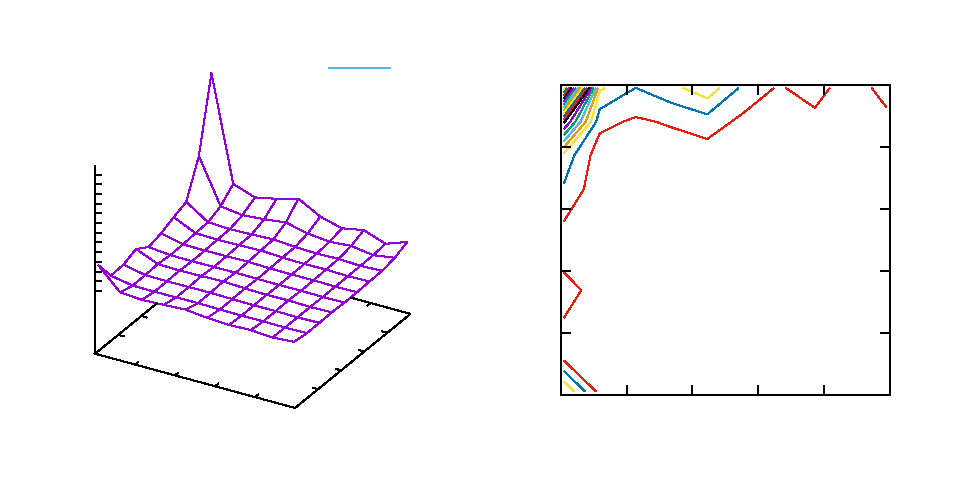
\includegraphics{images/plots/plot_30_51_1000}}%
    \gplfronttext
  \end{picture}%
\endgroup
